\documentclass[spanish]{book}
\usepackage{titlesec}

%Quitar páginas en blanco
\let\cleardoublepage\clearpage
\usepackage{etoolbox}
\makeatletter
\patchcmd{\@endpart}{\vfil\newpage}{\par}{}{}
\makeatother

%\usepackage[spanish]{babel} ¡Esto estaba interfiriendo con las flechitas de los \tikspicture

\renewcommand{\contentsname}{Índice}
\renewcommand{\partname}{Parte}

\titleformat{\chapter}[display]
{\normalfont\huge\bfseries}{}{0pt}{\Huge\thechapter.~}

\titleformat{name=\chapter,numberless}[display]
{\normalfont\huge\bfseries}{}{0pt}{\Huge}
\renewcommand{\chaptermark}[1]{\markboth{{} \thechapter: #1}{}}


%Cambiar el formato de los capítulos
\usepackage{titlesec}
\titleformat{\chapter}[display]
{\normalfont\huge\bfseries}{}{0pt}{\Huge\thechapter.~}
\titleformat{name=\chapter,numberless}[display]
{\normalfont\huge\bfseries}{}{0pt}{\Huge}
\renewcommand{\chaptermark}[1]{\markboth{{} \thechapter: #1}{}}

%Paquetes
\usepackage[left=4cm, right=4cm]{geometry}
\usepackage{palatino}%Fuente
\usepackage{graphicx}%Imágenes
\usepackage{float}%Imágenes
\usepackage{subcaption}%Imágenes
\usepackage{enumitem}%Listas
\usepackage{parskip}%Espacio entre párrafos
\usepackage{multicol}
\usepackage{amsthm}%Mate
\usepackage{amssymb}%Mate
\usepackage{amsmath}%Mate
\usepackage{tikz}%Mate (diagramas)
\usepackage{tikz-cd}
\usetikzlibrary{%
	matrix,%
	calc,%
	arrows,%
	shapes,
	decorations.markings
}
\usepackage[bookmarks,bookmarksopen,bookmarksdepth=3]{hyperref}%Links a lugares en el texto
\hypersetup{%colores
	colorlinks=true,
	urlcolor=blue,
	linkcolor=magenta,
	citecolor=blue,
	filecolor=blue,
	urlbordercolor=white,
	linkbordercolor=white,
	citebordercolor=white,
	filebordercolor=white
}

%Referencias
\usepackage[style=mla]{biblatex}
\addbibresource{bib.bib}

\theoremstyle{definition}
\renewcommand{\proofname}{Demostración}

\newtheorem*{defn}{Definición}
\newtheorem*{teo}{Teorema}
\newtheorem*{prop}{Proposición}
\newtheorem*{coro}{Corolario}
\newtheorem*{lema}{Lema}
\newtheorem*{obs}{Observación}
\newtheorem{ejer}{Ejercicio}
\newtheorem*{ejer*}{Ejercicio}
\newtheorem*{af}{Afirmación}
\newtheorem*{ejem}{Ejemplo}
\newtheorem*{pregunta}{Pregunta}

\newcommand{\R}{\mathbb{R}}
\newcommand{\Z}{\mathbb{Z}}
\newcommand{\N}{\mathbb{N}}
\newcommand{\C}{\mathbb{C}}
\newcommand{\Q}{\mathbb{Q}}
\newcommand{\Cinf}{C^\infty}

\DeclareMathOperator{\img}{img}
\DeclareMathOperator{\Arg}{Arg}

\title{Geometría Riemanniana}
\author{Semestre 2024-1}

\begin{document}
	\maketitle
	\phantomsection
	\addcontentsline{toc}{part}{\contentsname}
	\tableofcontents
	
	\chapter{Variedades Riemannianas}
	\section{Variedades diferenciables}
	\begin{defn}
		Una \textbf{variedad topológica} es un espacio topológico $M$ \textbf{localmente homeomorfo} a $\R^n$. Es decir, es un espacio topológico tal que para cualquier $p\in M$ existe una vecindad abierta $U\subseteq M$ de $p$, un abierto $V\subseteq\R^n$ y un  homeomorfismo $h:U\to V$. Decimos que $h$ es una \textbf{carta} y $U$ es una \textbf{vecindad coordenada}.
	\end{defn}
	Para definir el concepto de variedad diferenciable necesitamos primero definir alguna noción de diferenciablilidad en una variedad topológica. Comenzamos con el caso de funciones valuadas en los números reales. Consideremos el siguiente diagrama:
	\[\begin{tikzcd}
		U\subseteq M\arrow{r}{f} \arrow{d}[swap]{h} & \mathbb{R} \\
		V \subseteq \mathbb{R}^n \arrow[swap,dashed]{ur}{f \circ h^{-1}} 
	\end{tikzcd}\]
	La idea es que una función $f:M\to\R$ debe ser suave en $p\in M$ si la composición $f\circ h^{-1}$ es suave en $h(p)$. Pero hay un detalle: necesitamos que esta definición no dependa de la carta.
	
	Podría ser que un mismo punto $p$ estuviera en dos vecindades coordenadas $U_\alpha$ y $U_\beta$. ¿Es posible que $f\circ h^{-1}_\alpha$ sea suave y $f\circ h_\beta^{-1}$ no?
	\[\begin{tikzcd}
		&p\in U_\alpha\cap U_\beta\arrow{dl}[swap]{h_\alpha}\arrow{dr}{h_\beta}\\
		V_\alpha\arrow{rr}[swap]{h_\beta\circ h_\alpha^{-1}}&&V_\beta
	\end{tikzcd}\]
	Necesitamos agregar la condición de que las transformaciones de cambio de coordanas $h_\beta\circ h_\alpha^{-1}$ sean suaves. En est caso, si suponemos que $f\circ h_\beta^{-1}$ es suave, entonces también $(f\circ h_\beta^{-1})\circ(h_\beta\circ h_\alpha^{-1})=f\circ h_\alpha^{-1}$ también es suave (ya que la composición de dos funciones suaves es suave. Así, la composición de $f$ con cualquier carta coordenada queda suave.
	\begin{defn}
		Un \textbf{atlas} en un espacio topológico $M$ es una colección de cartas en $M$ tal que
		\begin{enumerate}
			\item[(A2)] Todo punto de $M$ está en alguna vecindad coordenada.
			\item[(A1)] Cualquier par de cartas se traslapa suavemente.
		\end{enumerate}
		Un atlas $\mathcal C$ en $M$ es \textbf{completo} si $\mathcal{C}$ contiene toda carta en $M$ que se traslapa suavemente con todas las cartas de $\mathcal{C}$.
	\end{defn}
	\begin{lema}
		Todo atlas en $M$ está contenido en un único atlas completo.
	\end{lema}
	\begin{proof}
		Sea $\mathcal{A}$ un atlas en $M$, y definamos
		\[\mathcal{A}'=\{h:U\subset M\to\R^n:h\text{ se tralsapa suavemente con todas las cartas en }\mathcal{A}\}\]
		Ahora observamos que (1) $\mathcal{A}'$ es un atlas, pues satisface (A1) trivialmente y (A2), que es claro si alguna de las cartas está en $\mathcal{A}$, y si no, basta componer con una en $\mathcal{A}$ y su inversa, reduciendo el dominio si es necesario. $\mathcal{A}'$ es maximal por definición. Ahora sea $\mathcal{C}$ otro atlas completo en $M$ tal que $\mathcal{A}\subseteq\mathcal{C}$. Como $\mathcal{C}$ satisface (A2), entonces $\mathcal{C}\subseteq\mathcal{A}'$ por definición de $\mathcal{A}'$. Y como $\mathcal{C}$ es completo, debe contener a todas las cartas en $\mathcal{A}'$.
		
	\end{proof}
	\begin{ejem}[de un atlas no completo]
		Tomemos $M=S^1\subset\C$ y el atlas dado por las funciones
		\begin{align*}
			\begin{aligned}
				h_1:S^1\backslash\{-1\}&\to\R\\
				z&\mapsto\Arg(z)
			\end{aligned}
			\qquad
			\begin{aligned}
				h_2:S^1\backslash\{1\}&\to\R\\
				z&\mapsto\Arg(z)
			\end{aligned}
		\end{align*}
		Que se traslapan suavemente y cubren a $S^1$. Ahora notemos que la carta
		\begin{align*}
			k:S^1\cap\{x+iy:y>0\}&\mapsto\R\\
			x+iy&\mapsto x
		\end{align*}
		también se traslapa suavamente con las otras dos.
	\end{ejem}
	\begin{defn}
		Una \textbf{variedad diferenciable} es una variedad topológica tal que cada cambio de coordenadas es suave. Además, el atlas debe se \textbf{maximal} en el sentido de que estén contenidas todas las cartas que sean compatibles con las de cualquier atlas dado. Es decir, no es posible añadir otra carta que sea compatible con las anteriores.
		
		Para una carta de la forma $h_\alpha(q)=(x_\alpha(q),y_\alpha(q))$, $U_\alpha\subseteq M$, $h_\alpha:U_\alpha\to V_\alpha\subseteq\R^2$, diremos que 
		\[x_\alpha:U_\alpha\subseteq M\to \R\]
		es una \textbf{función coordenada}. La carta $h_\alpha$ también se llama \textbf{sistema de coordenadas}.
	\end{defn}
	Ahora definamos funciones suaves entre variedades.
	\begin{defn}
		Una función $\phi:M\to N$ entre las variedades $M$ y $N$ es una \textbf{transformación suave} si para cualquier punto $p\in M$ existe una carta $h:U\to \R^m$ y una carta $k:V\to\R^n$ con $p\in U$ y $\phi(p)\in V\subseteq N$ tales que 
		\[\begin{tikzcd}
			&M\arrow{r}{\phi}\arrow[swap]{d}{h}&N\arrow{d}{k}\\
			&\R^m\arrow[dashed]{r}&\R^n
		\end{tikzcd}\]
		la composición $k\circ\phi \circ h^{-1}$ es suave. Una transformación suave con inversa suave se llama \textbf{difeomorfismo}.
	\end{defn}
	\begin{obs}
		La función $h_\alpha\circ h_\beta^{-1}$ es un difeomorfismo.
	\end{obs}
	\begin{ejem}[de una carta coordenada]
		Una esfera $S^2=\{(x,y,z)\in\R^3:x^2+y^2+z^2=1\}$ con el abierto
		\[U_1=\{(x,y,z)\in\R^3: x^2+y^2+z^2=1, z>0\}\]
		\[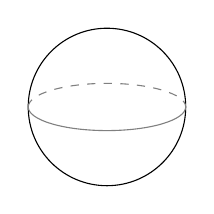
\begin{tikzpicture}
			% Outer circle
			\draw (0,0) circle (1);
			%3D
			\draw[gray] (-1,0) arc (180:360:1 and 0.3);
			\draw[gray,dashed] (-1,0) arc (180:0:1 and 0.3);
		\end{tikzpicture}\]
		y el homeomorfismo
		\[h_1(x,y,z)=(x,y).\]
	\end{ejem}
	\begin{ejem}[de un cambio de coordenadas]
		Tomemos un punto en $S^2$, por ejemplo $p=(\frac{1}{2},\frac{1}{2},\frac{1}{2})$, que está en $U_1$, y también en $U_2=\{(x,y,z)\in\R^3: x^2+y^2+z^2=1, y>0\}$ con $h_2=(x,z)$. Luego,
		\[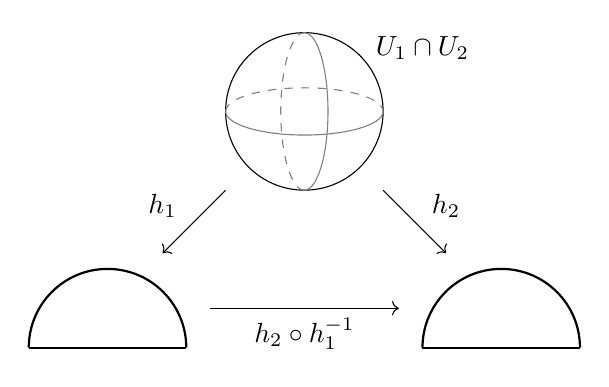
\begin{tikzpicture}
			% Sphere
			\draw (0,0) circle (1);
			\draw[gray] (-1,0) arc (180:360:1 and 0.3);
			\draw[gray,dashed] (-1,0) arc (180:0:1 and 0.3);
			\draw[gray,dashed] (0,-1) arc (270:90:0.3 and 1);
			\draw[gray] (0,1) arc (90:-90:0.3 and 1);
			\node at (1.5,0.8) {$U_1\cap U_2$};
			
			% Arrows and labels
			\draw[->] (-1,-1) -- (-1.8,-1.8);
			\node at (-1.8,-1.2) {$h_1$};
			\draw[->] (1,-1) -- (1.8,-1.8);
			\node at (1.8,-1.2) {$h_2$};
			\draw[->] (-1.2,-2.5) -- (1.2,-2.5) node[midway,below] {$h_2\circ h_1^{-1}$};
			
			% Left part
			\draw[thick] (-1.5,-3) arc (0:180:1);
			\draw[thick] (-1.5,-3) -- (-3.5,-3);
			
			% Right part
			\draw[thick] (1.5,-3) arc (180:0:1);
			\draw[thick] (1.5,-3) -- (3.5,-3);
		\end{tikzpicture}\]
		El cambio de coordenadas es $h_2\circ h_1^{-1}=(x,\sqrt{1-x^2-y^2})$, que es una función suave.
	\end{ejem}
	\begin{ejem}[El plano proyectivo real]
		En $\R^3\backslash\{(0,0,0)\}$ definamos la relación de equivalencia
		\[(x_1,y_1,z_1)\sim(x_2,y_2,z_2)\iff\exists\lambda\neq0\text{ tal que }(x_2,y_2,z_2)=\lambda(x_1,y_1,z_1)\]
		Como ejercicio se puede comprobar que en efecto se trata de una relación de equivalencia. El conjunto de clases de equivalencia se llama \textbf{plano proyectivo real} y de denota por $\R P^2$. A la clase de equivalencia de $(x_0,y_0,z_0)$ la denotamos $[x_0:y_0:z_0]$ y decimos que son las \textbf{coordenadas homogéneas} del punto.
		
		¿Cuáles serán las cartas?
		\begin{align*}
			\begin{aligned}
				U_0=\{[x:&y:z:]|x\neq0\}\\
				h_0:U_0&\to\R^2\\
				[x:y:z]&\mapsto\left(\frac{y}{x},\frac{z}{x}\right)
			\end{aligned}\qquad
			\begin{aligned}
				U_1=\{[x:&y:z:]|y\neq0\}\\
				h_1:U_1&\to\R^2\\
				[x:y:z]&\mapsto\left(\frac{x}{y},\frac{z}{y}\right)
			\end{aligned}\qquad
			\begin{aligned}
				U_2=\{[x:&y:z:]|z\neq0\}\\
				h_2:U_2&\to\R^2\\
				[x:y:z]&\mapsto\left(\frac{x}{z},\frac{y}{z}\right)
			\end{aligned}
		\end{align*}
		Observemos que $\R P^2=U_0\cup U_1\cup U_2$. Para encontrar los cambios de coordenadas, notemos que $h_1^{-1}=[u_1,1,v_1]$, de forma que $h_2\circ h_1^{-1}=h_2[u_1:1:v_1]=\left(\frac{u_1}{v_1},\frac{1}{v_1}\right)$, que es una función diferenciable.
		\[\begin{tikzcd}
			&U_1\cap U_2\arrow[swap]{ld}{h_1}\arrow{rd}{h_2}\\
			\R^2\arrow[swap]{rr}{h_2\circ h_1^{-1}}&&\R^2
		\end{tikzcd}\]
		Ahora definamos alguna función real-valuada en $\R P^2$ para ver si es suave. Tomemos el ejemplo de
		\begin{align*}
			f:\R P^2&\to \R\\
			f[x:y:z]=\arccos&\left(\frac{|z|}{\sqrt{x^2+y^2+z^2}}\right)
		\end{align*}
		que está bien definida ya que al multiplicar un vector en $\R^3\backslash\{(0,0,0\}$ por un escalar $\lambda$, éste se cancela. ¿Es suave? ¿Continua?
		
		Bueno, podemos darnos cuenta de que es continua cuando pensamos que el plano proyectivo es el hemisferio norte de la esfera identificando puntos antípodas en el ecuador. En este caso, casi todos los puntos del plano proyectivo tienen un único representante. Sólo los puntos en el ecuador podrían causar problema, pero la identificación por puntos antípodas en el ecuador nos permite construir vecindades de estos puntos pegando dos medias vecindades.
		\[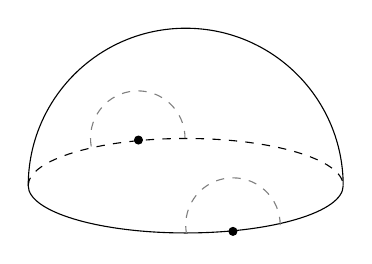
\begin{tikzpicture}[scale=2]
			% Outer circle
			\draw (-1,0) arc (180:0:1);
			%3D
			\draw (-1,0) arc (180:360:1 and 0.3);
			\draw[dashed] (-1,0) arc (180:0:1 and 0.3);
			
			\filldraw (-.3,.29) circle (0.025);
			\filldraw (.3,-.29) circle (0.025);
			
			\draw[gray,dashed] (-.6,.25) arc (190:0:0.3);
			\draw[gray,dashed] (.6,-.25) arc (0:190:0.3);
		\end{tikzpicture}\]
		Para saber si la función es suave, debemos llevar el problema a $\R^2$ usando las cartas coordenadas. Creemos que este ejemplo en particular no es suave…
		
		Tomemos mejor
		\[g[x:y:z]=\frac{ax+by+cz}{cx+dy+fz}\]
		Si $p\in U_2$,
		\begin{align*}
			g\circ h_2^{-1}(u_2,v_2)&=g[u_2:v_2:1]\\
			&=\frac{au_2+bv_2+e}{cu_2+dv_2+f}
		\end{align*}
		¿Cómo nos aseguramos de que no se puede hacer cero el denominador? Intentemos dar una función de la forma
		\begin{align*}
			G:\R P^2&\to\R P^1\approx\R\cup\{\infty\}\\
			[x:y:z]&\mapsto[ax+by+ez:cx+dy+fz]
		\end{align*}
		¡Hay elecciones de los coeficientes $a,\ldots,f$ que hacen que la función no sea suave!
	\end{ejem}
	\begin{ejer*}
		Consideremos para todo $r>0$ la aplicación $\varphi_r:\R\to\R$ dada por
		\begin{align*}
			\varphi_r(t)=
			\begin{cases}
				\begin{aligned}
					t\qquad&\text{si }t\leq0\\
					rt\qquad&\text{si }t\geq0
				\end{aligned}
			\end{cases}
		\end{align*}
		
		Muestre que los atlas $(\varphi_r)_{r>0}$ definen una familia no numerable de estructuras diferenciables sobre $\R$. ¿Las variedades diferenciables correspondientes son difeomorfas?
		\[\begin{tikzpicture}
			% Axes
			\draw[->] (-3,0) -- (3,0) node[right] {$t$};
			\draw[->] (0,-2) -- (0,3) node[above] {$\varphi_{1/2}(t)$};
			
			% Function plot
			\draw[blue, thick, domain=-2:0] plot (\x, \x);
			\draw[blue, thick, domain=0:3] plot (\x, 0.5*\x);
		\end{tikzpicture}\]
	\end{ejer*}
	\begin{proof}[Solución]
		Primero observemos que la función $\varphi_r$ es un homeomorfismo, ya que es continua y su inversa, $\varphi_{1/r}$, también. Al ser una única carta, los cambios de coordenadas son por vacuidad suaves, así que $\R$ con el atlas que consta de la carta $\varphi_r$ es una variedad diferenciable para toda $r$.
		
		Si $\R_r$ es la variedad con el atlas $\varphi_r$, ¿será que $\R_1$ es difeomorfa a $\R_{1/2}$? Intentemos dar un difeomorfismo:
		\begin{align*}
			f:\R_1&\to\R_{1/2}\\
			x&\mapsto\begin{cases}
				\begin{aligned}
					x\qquad&\text{si }x\leq0\\
					2x\qquad&\text{si }x\geq0
				\end{aligned}
			\end{cases}
		\end{align*}
		Claramente $f$ es biyectiva. ¿Será suave? Notemos que si consideramos esta función de $\R_1$ en $\R_1$ no lo es, pues tiene un pico en 0. Recordando nuestra definición de función suave entre variedades, consideremos el siguiente diagrama:
		\[\begin{tikzcd}
			&\R_1\arrow{r}{f}\arrow[swap]{d}{\varphi_1}&\R_{1/2}\arrow{d}{\varphi_{1/2}}\\
			&\R\arrow[dashed]{r}&\R
		\end{tikzcd}\]
		De hecho $\varphi_{1/2}\circ f\circ\varphi^{-1}_1=\varphi_{1/2}\circ f=id$, así que $f$ es suave. Y por un cálculo análogo, $f^{-1}$ también. Esta construcción se generaliza fácilmente para construir un difeomorfismo de $\R_1$ en $\R_r$, y con una simple composición, concluimos que todas estas variedades son difeomorfas entre sí.
	\end{proof}
	
	\section{Vectores tangentes}
	Recordemos que para el caso de superficies en $\R^3$ los vectores tangentes se pueden ver como el vector velocidad de una curva regular en la superficie. ¿Cómo podemos generalizar esta definición?
	\begin{defn}
		Sean $M$ una variedad diferenciable, $p\in M$ y $C^\infty(M,\R)$ el conjunto de funciones suaves $f:M\to\R$. Un \textbf{vector tangente} a $M$ en $p$ es un funcional $v:C^\infty(M,\R)\to\R$ con las propiedades de que
		\begin{itemize}
			\item \textbf{$\R$-lineal:} $v(\lambda f+\mu g)=\lambda v(f)+\mu v(g)$
			\item \textbf{Regla de Leibniz:} $v(f\cdot g)=v(f)g(p)+f(p)v(g)$
		\end{itemize}
	\end{defn}
	Este concepto generaliza la idea de \textit{derivada direccional}: cada vector tangente es un operador que actúa como una derivada direccional.
	
	\begin{obs}
		Sean $M$ una variedad diferenciable y $p\in M$. La colección de todos los vectores tangentes a $M$ en $p$ es un espacio vectorial con las siguientes operaciones:
		\begin{itemize}
			\item Elemento cero: $f\mapsto0$.
			\item Suma: $v+w:C^\infty(M,\R)\to\R$ tal que $f\mapsto v(f)+w(f)$
			\item Producto escalar. $\lambda v:C^\infty(M,\R)\to\R$ tal que $f\mapsto\lambda v(f)$
		\end{itemize}
	\end{obs}
	¿Cuál será una base de este espacio vectorial? Se nos antoja tomar los vectores canónicos en el dominio de la \textbf{parametrización} (la función inversa de la carta coordenada, cuyo dominio es $\R^n$).
	
	Consideremos una vecindad coordenada $U$ de $p\in M$ y la carta correspondiente
	\begin{align*}
		h:U\subset M&\to V\subset\R^n\\
		q&\mapsto (x^1(q),x^2(q),\ldots,x^n(q))
	\end{align*}
	Diremos que $x^i:U\subset M\to\R$ son las \textbf{funciones coordenadas}.
	
	Ahora tomemos una función suave en la variedad, $f:M\to\R$, y componemos con la parametrización para obtener
	\begin{align*}
		f\circ h^{-1}:V\subset\R^n&\to\R\\
		(u^1,u^2,\ldots,u^n)&\mapsto f\circ h^{-1}(u^1,u^2,\ldots,u^n)
	\end{align*}
	Esta función tiene una derivada direccional,
	\[\frac{\partial}{\partial x^i}(f):=\frac{\partial}{\partial u^i}\Big|_{h(p)}(f\circ h^{-1})\]
	Cuando variamos $f$, obtenemos un operador que es un candidato perfecto para ser un vector tangente. Resultará que éstos son una base del espacio tangente $T_pM$.
	\begin{lema}[No visto en clase, \cite{ONeill}]
		Sea $v\in T_pM$.
		\begin{enumerate}
			\item Si $f,g\in\Cinf(M,\R)$ son iguales en una vecindad de $p$, entonces $v(f)=v(g)$.
			\item Si $h\in\Cinf(M,\R)$ es constante, $v(f)=0$.
		\end{enumerate}
	\end{lema}
	\begin{lema}
		Sea $g:V\to\R$ suave, donde $V\subset\R^n$ es un conjunto abierto convexo que contiene al $0$. Entonces, existen funciones $g_i:V\subset\R^n\to\R$ suaves tales que
		\[g(u^1,\ldots,u^n)=g(0,\ldots,0)+\sum_{i=1}^ng_i(u^1,\ldots,u^n)u^i\]
		y además $g_i(0,\ldots,0)=\frac{\partial g}{\partial u^i}(0,\ldots,0)$
	\end{lema}
	\begin{proof}
		Proponemos
		\[g_i(u^1,\ldots,u^n)=\int_0^1\frac{\partial g}{\partial u^i}(tu^1,\ldots,tu^n)dt.\]
		Hagamos un poco más explícitas las cuentas hechas en clase. Cuando fijamos un punto $(u^1,\ldots,u^n):=q\in\R^n$, podemos ver la función $g(tq)$ como una función de $\R$ en $\R$. ¿Cuál es su derivada? Debemos usar la regla de la cadena pensando en la composición de "multiplicar por $t$" seguida de $g$:
		\[d_t g(tq)=d_{tq}g\cdot d_t(tq)=\nabla_{tq}g\cdot q\]
		Donde $\cdot$ es el producto de matrices (en este caso es el producto punto), y $\nabla g$ es el vector de derivadas parciales. Luego aplicamos el teorema fundamental del cálculo para obtener:
		\begin{align*}
			g(u^1,\ldots,u^n)-g_i(0,\ldots,0)&=\int_0^1\frac{dg}{dt}(tu^1,\ldots,tu^n)dt\\
			&=\sum_{i=1}^n\int_0^1\frac{\partial g}{\partial u^i}(tu^1,\ldots,tu^n)u^idt\\
			&=\sum_{i=1}^nu^i\int_0^1\frac{\partial g}{\partial u^i}(tu^1,\ldots,tu^n)dt
		\end{align*}
	\end{proof}
	Lo anterior se puede expresar así:
	\begin{equation}\label{ec1}
		g=g(0)+\sum g_iu^i
	\end{equation}
	\begin{teo}[\textbf{12}, \cite{ONeill}]\label{teo:base}
		Si $h(q)=(x^1(q),\ldots,x^n(q))$ es una carta coordenada de $M$ en $p$, entonces los vectores $\frac{\partial}{\partial x^1}, \ldots, \frac{\partial}{\partial x^n}
		$ son una base del espacio tangente. Más aún,
		\[v = \sum_{i=1}^n v(x^i) \frac{\partial}{\partial x^i} \qquad \text{para toda } v \in T_pM\]
	\end{teo}
	\begin{proof}
		Tomemos $f\in\Cinf(M,\R)$ y definimos $g:=f\circ h^{-1}$ para usar el lema. Suponiendo que $h(p)=0$, sustituyendo en \ref{ec1}, obtenemos que 
		\[f=f(p)+\sum f_ix^i\]
		donde $f_i=\int_0^1\frac{\partial f}{\partial x^i}(tq)dt$. Derivando esta expresión respecto a $x^i$ simplemente obtenemos
		\begin{equation}\label{ec2}
			\frac{\partial f}{\partial x^i}=f_i
		\end{equation}
		Ahora sea $v\in T_pM$ cualquier vector tangente. Al aplicar $f$ obtenemos:
		\begin{align*}
			v(f) &= v\left(f(p)+\sum_{i=1}^nf_ix^i\right) \\
			&= v\left(f(p)\right)+v\left(\sum f_i x^i\right) \\
			&=0+ \sum v\left(f_i x^i\right)\qquad\qquad\text{ya que }f(p)\text{ es constante} \\
			&=\sum v(f_i)x^i(p)+f_i(p)v(x^i)\qquad\text{Leibniz}\\
			&=0+\sum \frac{\partial f_i}{\partial x^i}x^i\qquad\qquad\text{ya que }h(p)=0\text{ y por }\ref{ec2}
		\end{align*}
		Ahora veamos que los vectores son linealmente independientes. Supongamos que
		\[w:=\sum\alpha_i\frac{\partial}{\partial{x^i}}\Bigg|_{p}=0\in T_pM\]
		Evaluando en $x^j\in\Cinf$,
		\[0=w(x^j)=\sum\alpha_i\frac{\partial x^j}{\partial{x^i}}\Bigg|_{p}=\alpha_j\]
	\end{proof}
	\section{Diferencial de una aplicación}
	Dadas dos variedades $M$ y $N$, la \textbf{diferencial} de una función $\phi:M\to N$ en $p\in M$ es de la forma
	\begin{align*}
		d\phi_p:T_pM&\to T_pN\\
		v&\mapsto d\phi_p(v)
	\end{align*}
	La asociación es bastante natural: $d\phi_p(v)$ manda una función $f\in\Cinf(N,\R)$ en $v(f\circ\phi)$.
	\[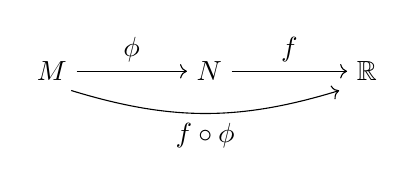
\begin{tikzpicture}
		\node (A) at (0,0) {$M$};
		\node (B) at (2,0) {$N$};
		\node (C) at (4,0) {$\R$};
		\draw[->] (A) -- node[above] {$\phi$}(B);
		\draw[->] (B) -- node[above] {$f$} (C);
		\draw[->, bend right=17] ([xshift=7pt]A.south) to node[below] {$f\circ\phi$} ([xshift=-10pt]C.south);
	\end{tikzpicture}\]
	\begin{obs}
		La diferencial es una transformación lineal.
	\end{obs}
	\begin{lema}[\textbf{14}, \cite{ONeill}]\label{lema:dif-coord}
		Sean $\phi:M\to N$ una transformación suave, $p\in M$ y $q=\phi(p)\in N$ con sistemas de coordenadas $h:U\subset M\to\R^m$ y $k:V\subset N\to\R^n$ tales que $h(p)=0$, y $k(q)=0$. Entonces,
		\[d\phi_p\left(\frac{\partial}{\partial x^j}\Big|_p\right)=\sum_{i=1}^n\frac{\partial(y^i\circ\phi)}{\partial x^j}(p)\frac{\partial}{\partial y^i}\Big|_{\phi p}\]
		Con funciones coordenadas  $h=(x^1,\ldots,x^m)$ y $k=(y^1,\ldots,y^n)$.
	\end{lema}
	\begin{proof}
		Definamos $v=\frac{\partial}{\partial x^j}\in T_pM$ y tomemos una función $g\in\Cinf(N,\R)$. Para encontrar $d\phi_p(v):=w$, usamos el \hyperref[teo:base]{teorema} anterior para expresar
		\begin{align*}
			w=\sum_{i=1}^nw(y^i)\frac{\partial}{\partial y^i}
		\end{align*}
		Y luego calculamos
		\[w(y^i)=v(y^i\circ\phi)=\frac{\partial}{\partial x^j}\Big|_py^i\circ\phi\]
	\end{proof}
	\begin{obs}
		Con toda formalidad, la expresión anterior es de la forma
		\[\frac{\partial}{\partial x^j}\Big|_py^i\circ\phi\\
		=\frac{\partial}{\partial u^j}\Big|_0y^i\circ\phi\circ h^{-1}	\]
	\end{obs}
	\begin{obs}\label{obs:dif-mat}
		Recordando que la diferencial es una transformación lineal entre los espacios tangentes, la matriz que la representa respecto a las bases $\left\{ \frac{\partial}{\partial x^1},\ldots,\frac{\partial}{\partial x^m}\right\}$ y $\left\{\frac{\partial}{\partial y^1},\ldots,\frac{\partial}{\partial y^n}\right\}$ es igual a la matriz que representa la derivada de la transformación en coordenadas respecto a las bases canónicas de los espacios euclideanos.
		
		Con todo detalle, sea $A=(a_{ij})$ la matrix de $n\times m$ coorespondiente a $d\phi_p$. Es decir,
		\[d\phi_p\left(\frac{\partial}{\partial x^j}\Big|_p\right)=\sum_{i=1}^na_{ij}\frac{\partial}{\partial y^i}\Big|_q\]
		De acuerdo al \hyperref[lema:dif-coord]{lema} anterior, $a_{ij}=\frac{\partial y^i\circ\phi\circ h^{-1}}{\partial x^j}$.
		
		La derivada de la transforamción en coordenadas es $d(k\circ\phi\circ h^{-1})_0$. Se trata de una transformación lineal $B:\R^m\to\R^n$. Recordando que las funciones coordenadas en el contradominio son $k=(y^1,\ldots,y^n)$, la representación matricial de $B$ es $\left(\frac{\partial y^i\circ\phi\circ h^{-1}}{\partial x_j}\right)_{ij}$.
	\end{obs}
	\section{Subvariedades}
	\begin{defn}
		Una \textbf{subvariedad} de $S$ de una variedad $M$ es una variedad tal que:
		\begin{enumerate}
			\item[\textit{i)}] Tiene la topología de subespacio de $M$.
			\item[\textit{ii)}] La inclusión $j:S\hookrightarrow M$ es suave y en cada punto $p\in S$ la diferencial de $j$ en $p$ $dj_p:T_pS\to T_pS$ es inyectiva.
		\end{enumerate}
	\end{defn}
	\begin{ejem}[Lemniscata]
		Pensamos una función $\alpha:\R\to L$, donde $L$ es la Lemniscata. Cuando le damos la topología inducida por $\alpha$, resulta que esta curva es una variedad. Sin embargo, no es una subvariedad de $\R^2$ con la topología usual de acuerdo a la definición que acabamos de dar.
		\[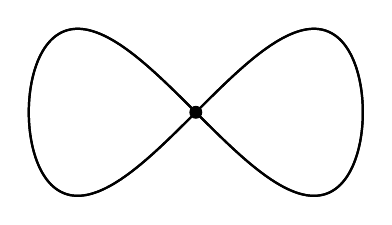
\begin{tikzpicture}[scale=1.5]
			
			\draw[thick, domain=0:360, samples=500] plot ({sqrt(2) * cos(\x)} , {sqrt(2) * cos(\x) * sin(\x)});
			\draw[thick, domain=0:360, samples=500] plot ({-sqrt(2) * cos(\x)} , {-sqrt(2) * cos(\x) * sin(\x)});
			
			\draw[fill=black] (0,0) circle (0.05);
		\end{tikzpicture}\]
	\end{ejem}
	\begin{ejem}[La gráfica del valor abosluto]
		Consideremos $S=\{(x,y)\in\R^2:y=|x|\}$, que es una subvariedad topológica de $\R^2$ con la topología usual.
		\[\begin{tikzpicture}
			% Axes
			\draw[->] (-3,0) -- (3,0) node[right] {$x$};
			\draw[->] (0,-.5) -- (0,3) node[above] {$|x|$};
			
			% Absolute value function plot
			\draw[blue, thick, domain=-3:3, samples=100] plot (\x, {abs(\x)});
		\end{tikzpicture}\]
		\begin{af}
			No existe ninguna estructura suave para $S$ tal que $S$ sea subvariedad de $\R^2$.
		\end{af}
		Supongamos que tenemos una carta coordenada $h$ en a algún atlas de $S$ y un vector $v\in T_pS$ cuya imagen bajo la diferencial $di_p$ es cero.
		\[\begin{tikzcd}
			S\arrow[hook]{r}{j}\arrow[swap]{d}{h}&\R^2\arrow{d}{id}\\
			\R\arrow[dashed]{r}&\R^2
		\end{tikzcd}\]		
		Notemos que la parametrización local es de la forma $h^{-1}(t)=(x,y)$ con $y=|x|$, o bien $y^2(t)=x^2(t)$. Derivando, $2y(t)y'(t)=2x(t)x'(t)$. Tenemos dos casos:
		\begin{itemize}
			\item Si $x(t)>0$, entonces $y(t)=x(t)$ y $y'(t)=x'(t)$. Tomando límite hacia el cero ya que las funciones son suaves, $y'(0)=x'(0)$.
			\item Si $x(t)<0$ entonces $y(t)=-x(t)$ y $y'(t)=-x'(t)$. Tomando límite, $y'(0)=x'(0)$.
		\end{itemize}
		\textit{*Falta concluir que ambas derivadas son cero*}
	\end{ejem} 
	\begin{obs}
		En \cite{Lee}, tenemos otra demostración de este hecho en el \textbf{Ejemplo 5.45}. Esencialmente, Lee usa la siguiente proposición:
		\begin{prop}
			Sean $M$ una variedad, $S\subset M$ una subvariedad, $p\in S$ y $v\in T_pM$. Entonces $v$ es un vector en $T_pS$ si y sólo si existe una curva suave $\gamma:J\to M$ cuya imagen está contenida en $S$, es suave como mapeo en $S$, y es tal que $0\in J$, $\gamma(0)=p$ y $\gamma'(0)=v$.
		\end{prop}
		Suponiendo que $S$ es una subvariedad, tendríamos una curva suave $\gamma:(-\varepsilon,\varepsilon)\to\R$ que en $0$ pasa por $(0,0)$ y su derivada no es cero, ya que el espacio tangente debe tener al menos un elemento no trivial. Si $\gamma(t)=(x(t),y(t))$, la función $y$ alcanza un mínimo en $t=0$, así que $y'(0)=0$. Y, como en la prueba que hicimos en clase, sabemos que $y^2(t)=x^2(t)$. Derivando dos veces, $y'(t)^2+y(t)y''(t)=x'(t)^2+x''(t)$. Evaluando en $t=0$, concluimos que $y'(t)=x'(t)=0$, pero esto es justo lo que no queríamos.
	\end{obs}
	
	
	
	\clearpage
	\section{Ejercicios 14-18 de agosto}
	Sea $M$ una variedad diferenciable de dimensión $m$ y $N$ una variedad diferenciable de dimensión $n$. Sea $p\in M$, $U$ una vecindad coordenada de $p$ con una carta $h:U\subset M\to\R^m$. Sea $q\in N$, $V$ una vecindad coordenada de $q$ con una carta $k:V\subset N\to\R^n$. A $M\times N$ le damos estructura de variedad, cuyas vecindades coordenadas son de la forma $U_\alpha\times V_\beta$, y cuyas cartas son de la forma 
	\begin{align*}
		h\times k:U_\alpha\times V_\beta&\to\R^m\times\R^n\\
		(p,q)&\mapsto \left(h(p),k(q)\right)
	\end{align*}
	\begin{enumerate}
		\item Las proyecciones 
		\begin{align*}
			\begin{aligned}
				\pi:M\times N&\to M\\
				(p,q)&\mapsto p
			\end{aligned}
			\qquad\text{ y }\qquad
			\begin{aligned}
				\sigma:M\times N&\to N\\
				(p,q)&\mapsto q
			\end{aligned}
		\end{align*}
		son suaves.
		
		\item Una transformación $\phi:P\to M\times N$ es suave si y sólo si $\pi\circ\phi$ y $\sigma\circ\phi$ son suaves.
		\item Para cada $(p,q)\in M\times N$ los subconjuntos
		\begin{align*}
			M\times q=\{(x,q)\in M\times N:x\in M\}\\
			p\times N=\{(p,y)\in M\times N:y\in N\}
		\end{align*}
		son subvariedades de $M\times N$.
		\item Para cada $(p,q)$,
		\begin{align*}
			\pi|_{M\times q}\text{ es un difeomorfismo }M\times q\to M\\
			\sigma|_{p\times N}\text{ es un difeomorfismo }p\times N\to N
		\end{align*}
	\end{enumerate}
	\begin{proof}[Solución]\leavevmode
		\begin{enumerate}
			\item Escogiendo un punto en $M\times N$ y una carta corrdenada $h\times k$, construimos el siguiente diagrama:
			\[\begin{tikzcd}
				M\times N\arrow{r}{\pi}\arrow[swap]{d}{h\times k}&M\arrow{d}{h}\\
				\R^m\times\R^n\arrow[dashed]{r}&\R^m
			\end{tikzcd}\]
			La flecha punteada manda $(x,y)\mapsto x$, que es suave.
			\item Para un punto en $P$ con carta coordenada $\ell$ tal que $h\times k$ es una carta de su imagen bajo $\phi$, tenemos:
			\[\begin{tikzcd}
				P\arrow{r}{\phi}\arrow[swap]{d}{\ell}&M\times N\arrow{d}{h\times k}\\
				\R^p\arrow[dashed]{r}&\R^m\times\R^n
			\end{tikzcd}\]
			Sabemos que $P$ es suave si y sólo si $(h\times k)\circ\phi\circ\ell^{-1}$ es suave.  Notemos que para $z\in\R^p$, $\left(h\times k)\left(\phi\left(\ell^{-1}(z)\right)\right)=\left(h\left(\phi\left(\ell^{-1}(z)\right)\right),k(\phi\left(\ell^{-1}(z)\right)\right)\right)$, de manera que la flecha punteada es suave cuando las dos funciones coordenadas son suaves, y de hecho, ¡éstas son las cartas coordenadas cuando componemos con las proyecciones!
			\item Primero debemos dar una estructura diferenciable para $M\times q$. Dado $(x,q)\in M\times q$ tomemos cualquier carta  $h:U_\alpha\to\R^m$ de $M$ que contenga a $x$ y definamos ${h\times q:U_\alpha\times\{q\}\to\R^m}$ simplemente por $(h\times q)(y,q)=h(y)$.
			
			Ahora veamos si la inclusión es suave mediante el siguiente diagrama:
			\[\begin{tikzcd}
				M\times q\arrow[hook]{r}{j}\arrow[swap]{d}{h\times q}&M\times N\arrow{d}{h\times k}\\
				\R^m\arrow[dashed]{r}&\R^m\times\R^n
			\end{tikzcd}\]
			Notemos que hemos usado la carta $h$ en dos lugares distintos. La flecha punteada es la inclusión $\R^m\hookrightarrow\R^m\times\R^n$, que es suave. Para ver que su diferencial es inyectiva, usamos la \hyperref[obs:dif-mat]{observación} de que la matriz que representa a la diferencial es la misma que la matriz de la derivada de la transformación en coordenadas, que es $\begin{pmatrix}
				id_{m}\\0_{n}
			\end{pmatrix}$, y en particular es inyectiva.
			
			\textbf{Otro camino}: supongamos que $v\in T_{M\times q}$ es tal que $dj_pv=0$. Para ver que $v=0$, tomemos $f\in\Cinf(M\times q,\R)$. Consideremos la función $\tilde{f}\in\Cinf(M\times N,\R)$ dada por $\tilde{f}(x,y)=f(x,q)$, que es suave ya que la derivada de $\tilde{f}\circ(h\times k)^{-1}$ es el vector $(df_p,0,\ldots,0)$. Luego, $v(f)=v(f\circ j)=dj_pv(\tilde{f})=0$.
			\item La restricción de una función suave a una subvariedad es suave. Para dar una demostración explícita, tomamos cartas coordenadas alrededor de algún punto para construir el siguiente diagrama:
			\[\begin{tikzcd}
				M\times q\arrow{r}{\pi|_{M\times q}}\arrow[swap]{d}{h\times q}&M\arrow{d}{h}\\
				\R^m\arrow[dashed]{r}&\R^m
			\end{tikzcd}\]
			La flecha punteada es la identidad. El caso de la función inversa es análogo.
		\end{enumerate}
	\end{proof}
	\begin{ejem}[de una variedad producto]
		Consideremos $S^1=\{(x,y)\in\R^2|x^2+y^2=1\}$ con el atlas
		\begin{align*}
			\begin{aligned}
				&h_N(x,y)=x\\
				&U_N=\{(x,y)\in S^1|y>0\}\\\\
				&h_O(x,y)=y\\
				&U_E=\{(x,y)\in S^1|x<0\}
			\end{aligned}
			\qquad
			\begin{aligned}
				&h_S(x,y)=y\\
				&U_S=\{(x,y)\in S^1|y<0\}\\\\
				&h_E(x,y)=y\\
				&U_E=\{(x,y)\in S^1|x>0\}
			\end{aligned}
		\end{align*}
		Que son las proyecciones al eje $x$ o $y$.
		\[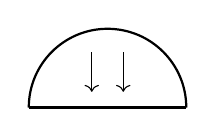
\begin{tikzpicture}
			\draw[thick] (1,0) arc (0:180:1);
			\draw[thick] (-1,0) -- (1,0);
			\draw[->] (-.2,0.7)--(-.2,0.2);
			\draw[->] (.2,0.7)--(.2,0.2);
		\end{tikzpicture}\]
		Ahora sea $S^1\times S^1$ con las cartas producto, que son de la forma
		\begin{align*}
			h_N\times h_N:U_N\times U_N\subset S^1\times S^1&\to\R\times\R\approx\R^2\\
			\left((x_1,x_2),(y_1,y_2)\right)&\mapsto\left(h_N(x_1,x_2),h_N(y_1,y_2)\right)=(x_1,y_1)
		\end{align*}
		Podemos definir un atlas análogo en esferas de cualquier dimensión proyectando cada hemisferio al plano que lo determina.
		\[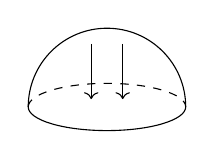
\begin{tikzpicture}[scale=1]
			\draw (-1,0) arc (180:0:1);
			\draw (-1,0) arc (180:360:1 and 0.3);
			\draw[dashed] (-1,0) arc (180:0:1 and 0.3);
			\draw[->] (-.2,0.8)--(-.2,0.1);
			\draw[->] (.2,0.8)--(.2,0.1);
		\end{tikzpicture}\]
		Para el caso de $S^2$, tenemos la figura de \cite{DoCarmo}:
		\begin{center}
			\includegraphics[width=0.5\linewidth]{fig1.png}
		\end{center}
		Con estas estructuras diferenciables podemos construir la variedad $S^p\times S^q$. (También podemos usar las proyecciones estereográficas desde el polo norte y el polo sur para cubrir a la esfera con sólo dos cartas).
	\end{ejem}
	
\section{Covectores}
\begin{defn}
	Una \textbf{1-forma} (\textbf{covector}) en un espacio tangente $T_pM$ es una función lineal $\omega:T_pM\to\R$.
\end{defn}
Las 1-formas (covectores) son elementos en el dual del espacio tangente $T_pM^*$, que llamaremos el espacio \textbf{cotangente}.
\begin{ejem}[Dos 1-formas en $(T_p\R^2)^*$]
	Dada una curva $\alpha:I\subset\R\to\R^2$ tal que $\alpha(0)=(x_0,y_0)$ y $\alpha'(0)=(v_1,v_2)$, tenemos las 1-formas (covectores)
	\begin{align*}
		\begin{aligned}
			dx:T_{(x_0,y_0)}\R^2&\to\R\\
		v=\alpha'(0)&\mapsto v_1
		\end{aligned}
		\qquad
		\begin{aligned}
			dy:T_{(x_0,y_0)}\R^2&\to\R\\
			v=\alpha'(0)&\mapsto v_1
		\end{aligned}
	\end{align*}
	Y resultará que cualquier $\omega\in T_(x_0,y_0)\R^2$ es de la forma $\omega=adx+bdy$. Es decir:
	\begin{align*}
		\omega:T_{(x_0,y_0)}\R^2&\to\R\\
		(v_1,v_2)&\mapsto av_1+bv_2
	\end{align*}
\end{ejem}
Ahora consideremos un vector tangente a una variedad $M$ en algún punto $p$ que en coordenadas locales se exprese como
\[v_p=a_1(p)\frac{\partial}{\partial x^1}\Big|_p+\ldots+a_n(p)\frac{\partial}{\partial x^n}\Big|_p\]
Si $\omega\in(T_pM)^*$, por linealidad tenemos
\[\omega(v_p)=a_1(p)\omega\left(\frac{\partial}{\partial x^1}\Big|_p\right)+\ldots+a_n(p)\omega\left(\frac{\partial}{\partial x^n}\Big|_p\right)\]
\begin{obs}
	Tendremos que
	\[dx_p^i\left(\frac{\partial}{\partial x^j}\Big|_p\right)=\begin{cases}
	1\qquad\text{si }i=j\\
	0\qquad\text{si }i\neq j
	\end{cases}\]
\end{obs}
\begin{obs}
	Las 1-formas (covectores) $dx^1,\ldots,dx^n$ son una base del espacio cotangente $(T_pM)^*$.
\end{obs}

\section{Campos vectoriales}
\begin{defn}[Informal]
	Un \textbf{campo vectorial} es una correspondencia que a cada $p\in M$ le asocia un vector tangente $v\in T_pM$, y varía suavemente sobre la variedad.
\end{defn}
Primero especifiquemos qué quiere decir la suavidad de un campo vectorial. Consideremos un vector tangente $v_p$ a una variedad $M$ anclado en el punto $p\in M$. Hemos visto que que deben existir coeficientes $a_i(p)$ tales que
\[v_p=a_1(p)\frac{\partial}{\partial x^1}\Big|_p+\ldots+a_n(p)\frac{\partial}{\partial x^n}\Big|_p\]
Suponiengo que $v_p$ es un elemento de un campo vectorial, podemos variar el punto en el que está anclado el vector para obtener otros vectores $v_q$ que se expresan análogamente como
\[v_q=a_1(q)\frac{\partial}{\partial x^1}\Big|_q+\ldots+a_n(q)\frac{\partial}{\partial x^n}\Big|_q\]
Decimos que un campo vectorial es \textbf{suave} si las funciones $a_1,\ldots,a_n:U\subset M\to\R$ son suaves.
\begin{obs}
	Para definir formalmente un campo vectorial como una función entre dos conjuntos, primero debemos construir el haz tangente.
\end{obs}
\begin{obs}
	Denotaremos al conjunto de campos vectoriales en una variedad por $\mathfrak{X}(M)$
\end{obs}
\section{Formas diferenciales}
Ahora construimos el concepto dual al de campo vectorial para covectores.
\begin{defn}
	Una \textbf{1-forma diferencial} en una variedad suave $M$ es una función que a cada punto $p\in M$ y a cada vector tangente $v_p\in T_pM$ le asocia un número $\omega(p,v_p)$.
\end{defn}
Localmente,
\[\omega(p,v_p)=\sum_{i=1}^na_i(p)dx^i_p(v_p)\]
con $a_i:U\subset M\to\R$ suave para toda $i$. Una expresión más sencilla es $\omega=\sum a_idx^i$.
\begin{obs}
	Dado un campo vectorial $V$ y una 1-forma diferencial $\omega$ en $M$, podemos calcular
	\[p\mapsto V_p\mapsto\omega_p(V_p)\in\R\]
	Este número lo denotaremos, abusando de notación por
	\[\omega(V):M\to\R\]
\end{obs}
\section{Corchete de Lie}
Dado un campo vectorial $V$ en una variedad $M$, es posible verlo como una función
\begin{align*}
	\begin{aligned}
		V:\Cinf(M,\R)\to\\
		f:M\to\R
	\end{aligned}
	\begin{aligned}
		\Cinf(M,\R)\\
		v(f):M&\to\R\\
		p&\mapsto v_p(f)
	\end{aligned}
\end{align*}
\chapter{Referencias}
	\printbibliography[heading=none]
\end{document}